\documentclass[../../main.tex]{subfiles}
\begin{document}
\subsection*{1.2}
Quattro cariche positive poste ai vertici di un quadrato di lato 2a = 10cm di valore $q = 10^{-8}C$.
\\a) Calcolare la forza esercitata dalle altre tre cariche su quella posta nel vettore (a,a) e le espressioni del potenziale e del campo elettrostatico lungo l'asse x.
\\b) Calcolare inoltre l'energia cinetica con la quale passa per il centro un elettrone abbandonato con velocità nulla in un punto dell'asse x distante $x_0 = 2a$ dal centro. 
\\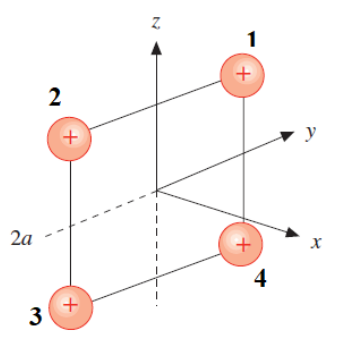
\includegraphics[scale=0.5]{e_1_2.png}
\subsubsection*{Formule utilizzate}
$\vec{F_{i,j}} = \frac{q_iq_j}{4\pi\epsilon_0r_{i,j}^2}\vec{u_{i,j}}$
\\$\vec{E_i} = \frac{q}{4\pi\epsilon_0r_i^2}$
\\$V(P) - V(\infty) = \int_x^\infty \vec{E}d\vec{s}$
\\$\vec{E} = \left(-\frac{\delta v}{\delta x}, -\frac{\delta v}{\delta y},-\frac{\delta v}{\delta z}\right)$
$\Delta E_k + \Delta U_{elettrone} = 0 $
\\$\Delta E_k = \frac{e}{4\pi\epsilon_0}\left[\frac{4q}{\sqrt{sa^2}}- \frac{4q}{\sqrt{2a^2 + 4a^2}}\right]$
\subsubsection*{Soluzione punto a}
Calcolo della forza:
\\Applico la formula per le 3 particelle
\\con $q_i = q_j = q $ 
\\$\vec{F_{2,1}} = \frac{q^2}{4\pi\epsilon_0r_{2,1}^2}\vec{u_{y}}$
$\vec{F_{3,1}} = \frac{q^2}{4\pi\epsilon_0r_{3,1}^2}\vec{u_{y,z}}$
$\vec{F_{2,3}} = \frac{q^2}{4\pi\epsilon_0r_{2,3}^2}\vec{u_{z}}$
\\\\Applico il teorema di sovrapposizione degli effetti:
\\$\vec{F} = \vec{F_{2, 1}} +\vec{F_{3, 1}} + \vec{F_{3, 2}}$
\\\\Calcolo del potenziale e del campo elettrostatico
\\$\vec{E_1} = \frac{q}{4\pi\epsilon_0r_1^2}$
$\vec{E_2} = \frac{q}{4\pi\epsilon_0r_2^2}$
$\vec{E_3} = \frac{q}{4\pi\epsilon_0r_3^2}$
$\vec{E_4} = \frac{q}{4\pi\epsilon_0r_4^2}$
\\con $r_1 = r_2 = r_3 = r_4 = \sqrt{2a^2+x^2}$
\\$\vec{E} = \vec{E_1} +\vec{E_2} + \vec{E_3} +\vec{E_4} = \frac{4q}{4\pi\epsilon_0r^2}\frac{x}{r}\vec{u_x}$
\\$V(P) - V(\infty) = \int_x^\infty \vec{E}d\vec{s}$
\\$V(P) = \frac{4q}{4\pi\epsilon_0}\int_x^\infty \frac{x}{r^3}dx = \frac{4q}{4\pi\epsilon_0}\frac{1}{\sqrt{2a^2+x^2}}$
\\$\vec{E} = \left(-\frac{\delta v}{\delta x}, -\frac{\delta v}{\delta y},-\frac{\delta v}{\delta z}\right)$

\subsubsection*{Soluzione punto b}
Calcolare l'energia cinetica di un elettrone con velocità nulla nel punto (2a, 0, 0) che passa in O.
\\$\Delta E_k + \Delta U_{elettrone} = 0 $
\\$\Delta E_k = \frac{e}{4\pi\epsilon_0}\left[\frac{4q}{\sqrt{sa^2}}- \frac{4q}{\sqrt{2a^2 + 4a^2}}\right]$
\newpage

\end{document}